\chapter{Problem Analysis}
Imagine sitting at a restaurant with your significant other and eating a delicious dinner and you notice a song they are playing, you quite enjoy the music, but both you and your partner do not know which song it is. To figure out which song it is, there are various options. One of the options is to ask the staff which song it is. This solution may be fast but a little bit tedious. Another option is to go through all the songs in a music app, this solution isn't the most effective way, though it spares you from an unwanted conversation. With modern technology you are able to download apps such as Shazam, which takes the good parts of both possibilities, you get spared from an unwanted conversation and it is quite fast.\\
Shazam is an app with the purpose of recognising songs from a recording. The app is able to recognise a song even if ambient noise is present, such as in a restaurant or a car. When Shazam recognises a song, it gives the user the title of the track, the artist and the ability to stream the song on multiple different music platforms. Shazam generates an audio fingerprint from which it can compare and match with songs in the database. \cite{ShazamDescription} \\
Another use case for audio fingerprinting is identification of copyrighted materials. This can be useful for social media where users can upload material freely, since the social media will be economically responsible if copyrighted material is shared on their platform. 
This use case comes with several challenges. For instance, the audio can be compressed. The end user may not hear the difference between the compressed audio and the original recording, but it is still covered by copyright. Furthermore, the users may try to avoid identification systems by adding inaudible noise. This means that the audio fingerprinting system must have the ability to recognise audio even though the waveform is modified. \cite{haitsma2003highly}

\section{Audio Fingerprinting Process}
An audio fingerprinting system can be generally be split into five parts.
\begin{itemize}
    \item \textbf{Audio recording:} Where the audio is digitised.
    \item \textbf{Filtering:} Removes the unwanted information of the recorded signal.
    \item \textbf{Generate fingerprint:} Generates the fingerprint needed to recognise the song.
    \item \textbf{Compare fingerprint to a database:} The generated fingerprint is compared to the fingerprints in the database.
    \item \textbf{Present the track information:} When the fingerprint is matched the relevant information is presented to the user.
\end{itemize}
This is illustrated in \autoref{fig:Fingerprint_process}.
These parts will be further explained in the next few sections.
   
\begin{figure} [H]
    \centering
    \begin{tikzpicture}[node distance = 4cm]
        \tikzstyle{box} = [rectangle, minimum width=3cm, minimum height=1cm, text centered, text width=3cm, draw=black]
        \tikzstyle{line} = [draw, -latex']
        \node (sampling) [box] {Audio recording};
        \node (filtering) [box, right of=sampling] {Filtering};
        \node (fingerprint) [box, right of=filtering] {Generate fingerprint};
        \node (compare) [box, below of=filtering, node distance =3cm] {Compare fingerprint to a database};
        \node (TrackInfo) [box, below of=sampling, node distance =3cm] {Present the track information};
        
        \path [line] (sampling) -- (filtering);
         \path [line] (filtering) -- (fingerprint);
        \path [line] (fingerprint) |- (compare);
         \path [line] (compare) -- (TrackInfo);
     \end{tikzpicture}
    \caption{The process of which an audio fingerprinting system uses audio recordings, filters the recordings, generates audio fingerprints, matches fingerprints and presents the user with the information.}
    \label{fig:Fingerprint_process}
\end{figure}


\subsection{Audio Fingerprinting}
To generate an audio fingerprint one might look at the semantics of a song such as genre and composition. Genres are generally difficult to quantify since they change as cultures change and sometimes overlap. Furthermore, there are almost endless ways to compose a song, hence it is also hard to quantify. Therefore it is not feasible to generate a audio fingerprint using semantics.\\

Another approach to generate an audio fingerprint for a piece of music, could be to consider getting knowledge of what songs and music consist of, and what sound really is.
Sound is created because of vibrations causing displacements and oscillations of molecules in a medium such as air, which can be considered as sound waves. These vibrations could for instance be caused from playing a guitar or the triangle. These waves can for instance be intercepted by the human ear or a microphone. The human ear can intercept frequencies between 20Hz and 20kHz, therefore when working with music, it is only relevant to work within this spectrum. \cite[21]{Meinard2015Fundamentals}\\
When recording audio, with a microphone, the audio signal becomes an electrical signal and the output would be changes in amplitude over time.

\begin{figure}
    \centering
    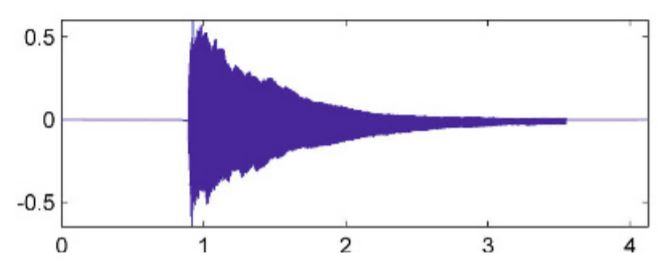
\includegraphics[width=0.8\textwidth]{figures/toneC4time.JPG}
    \caption{The tone C\textsubscript{4} played on a piano, in time domain}
    \label{fig:toneC4time}
\end{figure}

Considering only at the output in the time domain, it can be difficult to find patterns in the recording of the audio input using basic knowledge in music theory, such as tones and their defined frequencies. \\

Instead of looking at change in amplitude over time for an electrical signal, it is possible to look at changes in amplitude depending on frequencies for the input. This can be done by using the Discrete Fourier Transform (DFT), which transforms, for instance, an electrical signal in the time domain(Figur ovenover) to the complex frequency domain(Figur nedenunder).

\begin{figure}
    \centering
    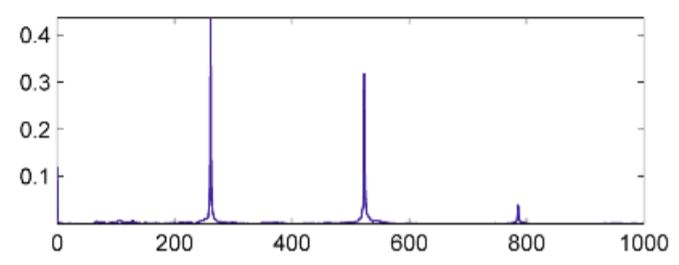
\includegraphics[width=0.8\textwidth]{figures/toneC4freq.JPG}
    \caption{Fourier transform of the audio recording of the tone C\textsubscript{4} played on a piano}
    \label{fig:toneC4freq}
\end{figure}

This is beneficial because different tones consists of defined/specific frequencies. For instance the tone C\textsubscript{4} played on a piano corresponds to $261.6 \si{Hz}$ \cite[29]{Meinard2015Fundamentals}.

\subsection{Filtering}
When recognizing music, there is often a bit of noise involved. The noise involved can be in the form of background speech, the motor of a car, generated noise from speakers ect. To remove the noise, a filter is used. The filter needs to be optimized so it only filters out the noise part of the signal and keeps the “clean” version of the song intact.\\

There are also different ways of encoding music, such as MP3 and GSM. The 2 different files compress the same music differently which results in the decoding of the song will be different. Nevertheless, the program will need to be able to recognize the song and generate the same fingerprint from both versions of the song.

\subsection{Search Algorithm}
When the fingerprint of a song has been generated, the fingerprint has to be matched to the track information in the database. The database can potentially consist of millions of fingerprints. When the database is so large it is not effective to brute force a match, therefore an optimized search algorithm is needed. However this will not be explored further in this project. \cite{haitsma2003highly} 

The program works by recording a sufficient amount of a song and then filtering noise from the recording. 
Thereafter an audio fingerprint is generated with mathematical models and theories. This fingerprint is then used to identify a song, by comparing and matching the fingerprint with an already generated database of fingerprints. If a match is found, the user is presented with the relevant information regarding the song. This process is illustrated in \autoref{fig:Fingerprint_process}. \cite{ShazamDescription}\\

Shazam is useful since it finds music simply and fast. It is not only the users which the app benefits, music artists also have benefits which consist of making their music more known, and therefore become more popular in the music industry. \cite{wang2003industrial} 







\section{Problem Statement}